\section{Physical principles}
\subsection{Hyperfine structure and Zeeman splitting}
This section is based on the detailed elaborations in \cite{staatsex}.\\
The fine structure levels of the atomic spectrum, which splits the basic levels into sub-levels due to spin-orbit interaction, can be shown to be split into even finer levels, whose energetic distances are roughly three orders of magnitude smaller than those of the fine structure. This is called the 'hyperfine structure' and is mainly caused by the interaction of the nuclear magnetic dipole and quadrupole moment and the magnetic field of the shell electrons. Its structure for the two Rubidium isotopes that are used in this experiment can be seen in figure \ref{fig:hyperfinestructure}.\\

As the nucleus is charged and, expressed as the nuclear spin $\vec{I}$, has angular momentum, it also has a magnetic moment, which is $\vec{\mu}_I=\frac{g_I\mu_K}{\hbar}\vec{I}$, where $g_I$ is the g-factor of the nucleus and $\mu_K$ is the nuclear magneton. 

With the total angular momentum of the electrons $\vec{J}$, the total angular momentum of the atom can be written as

\begin{equation}
\vec{F}=\vec{J}+\vec{I},\qquad \lvert I-J\rvert\le F \le I+J
\end{equation}

The energy difference between hyperfine structure levels can then shown to be

\begin{equation}
\Delta E_{HFS}=-\vec{\mu}_I\cdot\vec{B}_J=\frac{A}{2}(F(F+1)-J(F+1)-I(I+1))
\end{equation}

where $A=\frac{g_I\mu_KB_J}{\sqrt{J(J+1)}}$ is the hyperfine constant. Neighboring levels thus have an energy difference of

\begin{equation}
\Delta E_{HFS}(F+1)-\Delta E_{HFS}(F)=A(F+1)
\label{eq:hfslevels}
\end{equation}

This structure for the rubidium isotopes used in this experiment can be seen in figure \ref{fig:hfslevels}.\\

\begin{figure}[H]
\centering
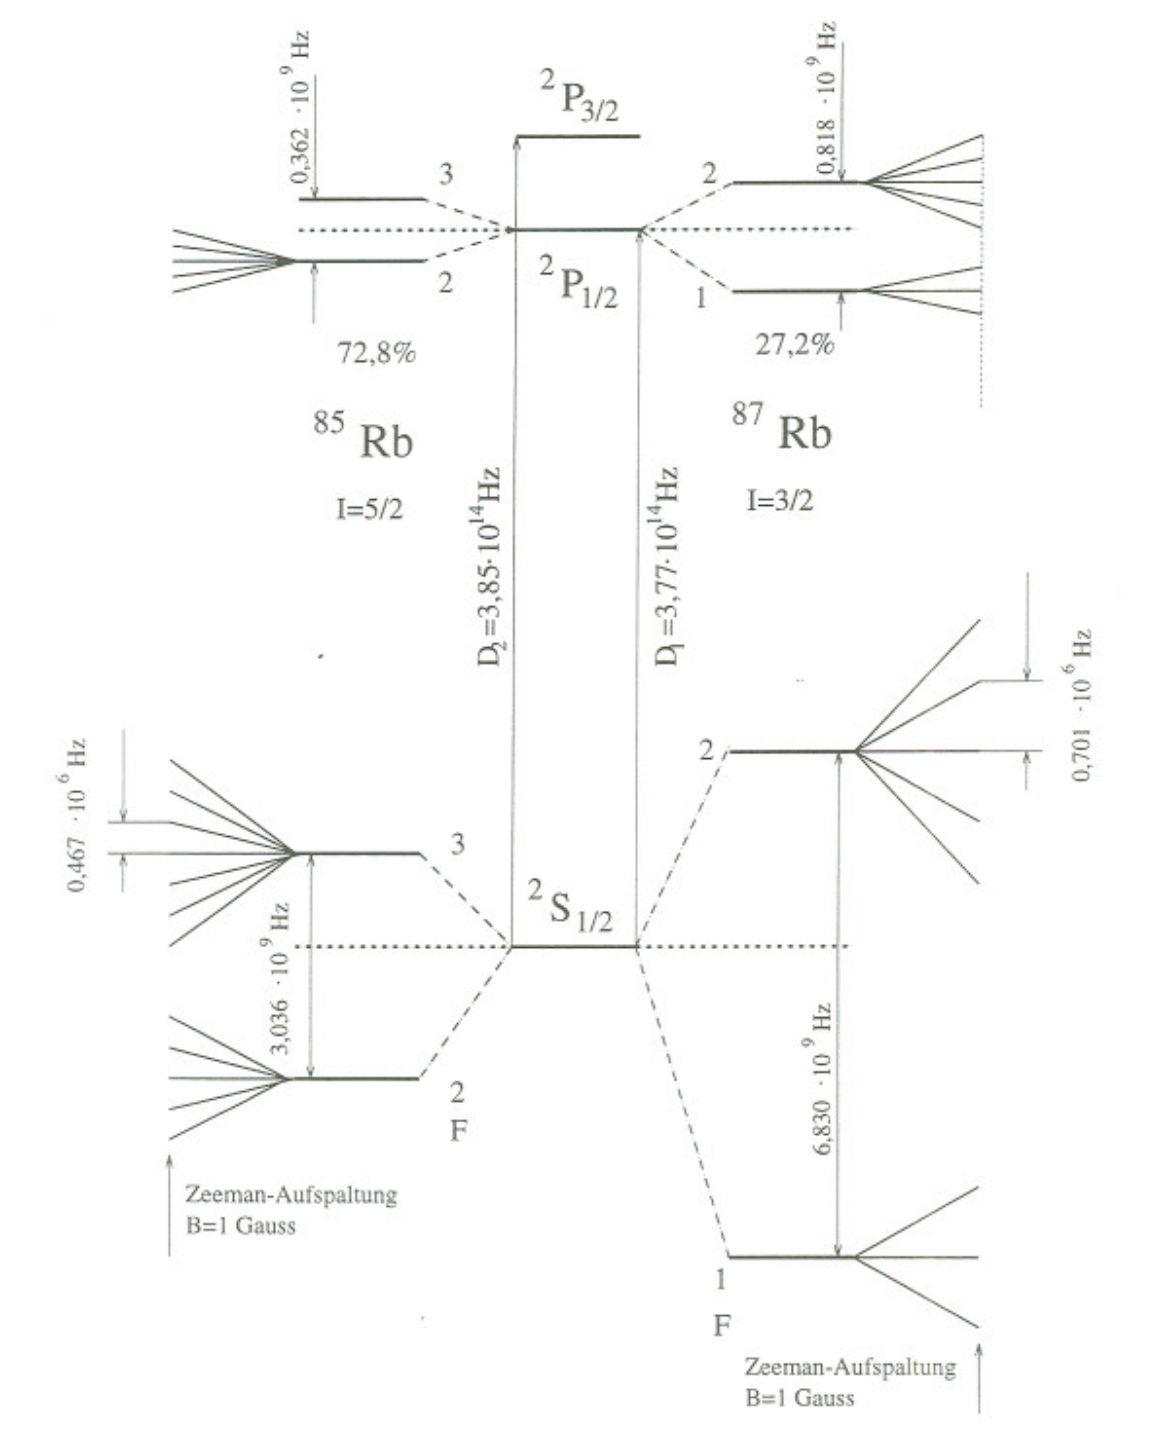
\includegraphics[width=1.0\linewidth]{graphics/hyperfinestructure}
\caption[Hyperfine structure of Rubidium]{The hyperfine structure of the two isotopes of Rubidium used in the experiment. The hyperfine levels in turn are split due to the Zeeman effect caused by an external field of $B=1$ G. \cite{staatsex}}
\label{fig:hyperfinestructure}
\end{figure}

\begin{figure}[H]
\centering
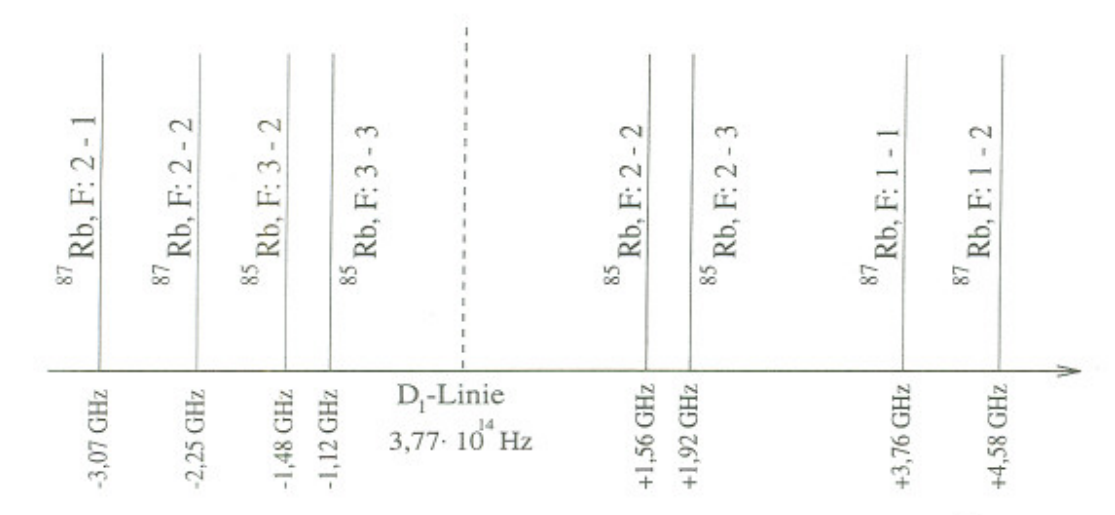
\includegraphics[width=1.0\linewidth]{graphics/hfslevels}
\caption[Hyperfine structure energies]{Energies of a set of hyperfine levels of the two isotopes used in the experiment. \cite{staatsex}}
\label{fig:hfslevels}
\end{figure}

These hyperfine levels can in turn be split into $2(F+1)$ sub-levels in the presence of an external magnetic field. The according quantum number is $-F\le m_F\le F$. As long as the magnetic field is weaker than the spin-orbit coupling or, in other terms, $g_J\mu_BB_0\ll A$, this is called the Zeeman effect. The effect for larger fields, where the spin-orbit coupling is disrupted, is called Paschen-Back effect.\\
For the Zeeman effect, the energy difference of the levels is
\begin{equation}
\Delta E_{Zeeman}=\frac{g_J}{2(I+\frac{1}{2})}\mu_BB_0
\label{eq:zeemanlevels}
\end{equation}
where $\mu_B$ is the Bohr magneton.

\subsection{Optical pumping}
In general, pumping refers to constantly transferring electrons into higher energy levels until significantly more electrons are in the higher than in the lower state. This is called population inversion.\\
In the case of this experiment, this is done using a laser diode. As the goal is to examine magnetic fields using the Zeeman splitting, a way must be found to create population inversion within a single non-degenerate hyperfine structure level. Normally, electrons are equally distributed between said levels.\\
The selection rules for transitions
\begin{equation}
\begin{aligned}
\Delta F&=0,\pm 1 \qquad (F=0\nleftrightarrow F=0)\\
\Delta m_F&=0,\pm 1
\end{aligned}
\end{equation}

allow for a convenient way to change that. If only $\sigma^+$-polarized light is used, only transitions with $\Delta m_F=+1$ are caused. Since the following decay is random within the bounds of the transition rules, the laser will pump all electrons into the $^2S_{1/2}$ state with $m_F=+2$, $F=2$ for $^{87}Rb$ and $m_F=+3$, $F=3$ for $^{85}Rb$. Figure \ref{fig:zeemanpumping} illustrates this for two exemplary transitions.\\
Mathematically, this process can be described as 
\begin{equation}
\left(\frac{dn}{dt}\right)_P=\frac{N-n}{T_P}
\label{eq:pumpingtime}
\end{equation}
where $n$ is difference of the levels in the two-level system, $N$ the overall number of atoms in the system and $T_P$ the characteristic pumping time of the system.
\begin{figure}[h]
\centering
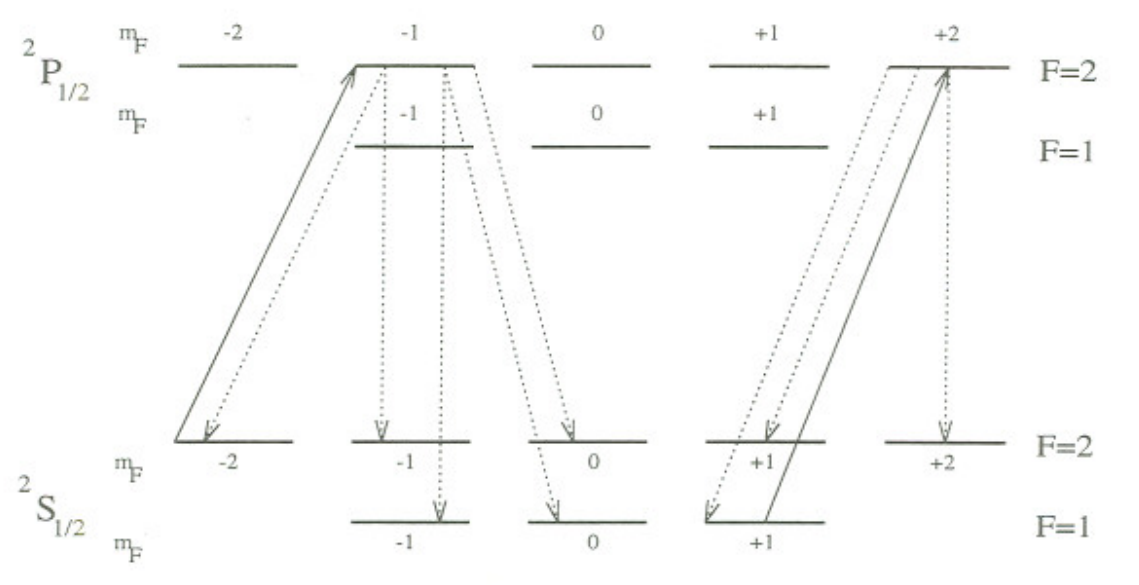
\includegraphics[width=1.0\linewidth]{graphics/zeemanpumping}
\caption[Optical pumping]{Optical pumping for $^{87}Rb$. The $\sigma^+$ polarized light can only cause transitions with $\Delta m_F=+1$, thus achieving the desired pumping effect.}
\label{fig:zeemanpumping}
\end{figure}
\subsection{Relaxation processes}
The desired pumping effect is counteracted mainly by three relaxation effects:
\paragraph{Diffusion to the wall:}
Upon hitting the glass containment, the rubidium atoms may lose their polarization. This process is inhibited by a buffer gas, which limits the mean free path of the atoms.
\paragraph{Collisions with the buffer gas:}
The rubidium atoms may use their polarization due to collisions with the buffer gas. The cross section of this event depend highly on what kind of gas is used. Best results are achieved with noble gases - in the case of this experiment, krypton was used.
\paragraph{Spin exchange}
When rubidium atoms collide, they may interchange their spins. While the overall polarization is preserved, the decoupling of nuclear and electron spins lead to a faster relaxation time. Much more detailed elaborations can be found in \cite{happer}.\\

Overall, the relaxation can be described by the following differential equation
\begin{equation}
\left(\frac{dn}{dt}\right)_R=-\frac{n}{T_R}
\label{eq:relaxationtime}
\end{equation}
where $T_R$ is the characteristic relaxation time. A value of $T^{theo}_R=\unit{6.5}{ms}$ is given in \cite{staatsex}. The overall process of polarization orientation is thus the sum of equations \ref{eq:pumpingtime} and \ref{eq:relaxationtime}:
\begin{equation}
\left(\frac{dn}{dt}\right)_O=\left(\frac{dn}{dt}\right)_P+\left(\frac{dn}{dt}\right)_R=\frac{N}{T_P}-n\left(\frac{1}{T_P}+\frac{1}{T_R}\right)
\end{equation}

The solution of this equation is an exponential
\begin{equation}
n(t)\propto e^{-\frac{t}{\tau}}
\label{eq:orientationexponential}
\end{equation}

where 
\begin{equation}
\tau=\frac{1}{T_P}+\frac{1}{T_R}\label{eq:tauIrelation}
\end{equation}
\subsection{Larmor precession of the spin}
If the ensemble is polarized along a certain magnetic field and one component of said field is suddenly set to zero, the polarization precesses around the remaining field. The precession frequency is
\begin{equation}
f_L=\frac{g_F\mu_B}{h}\cdot B =: \alpha\cdot B
\label{eq:precessionfreq}
\end{equation}
where $g_F$ are the Landé factors for the rubidium isotopes, quantified by Baur \cite{staatsex} as $g_F(^{85}Rb)=\nicefrac{1}{3}$ and $g_F(^{87}Rb)=\nicefrac{1}{2}$. The proportionality constant between the frequency and the remaining magnetic field thus is 
\begin{equation}
\alpha(^{85}Rb)=\unitfrac[4.665]{\kilo\hertz}{\micro\tesla}\quad \alpha(^{87}Rb)=\unitfrac[6.998]{\kilo\hertz}{\micro\tesla}
\end{equation}

